\chapter{時間軸セグメントを導入したHTM}
\section{提案モデルの概要}
従来のHTMは1つ前の時刻におけるパターンを表現するセルのみとの接続を持つように学習していたが、前章で述べたように長期依存考慮を要する予測タスクに対して脆弱性があった。
そのためHTMの性能を改善するためにHTMに時間軸セグメントを導入することによって、複数前の時刻におけるパターンを表現するセルとの接続も持つように学習させた。

この改良の重要な点は新たに接続をもつようになった時刻の範囲においてのみに長期依存関係を保持できるようになったということではない。
HTMの学習において予測状態に遷移するセルに関して適切な密度を保持し続けることは重要な要素であるが、改良したHTMは複数前の時刻にわたって接続を学習することによってセルの状態遷移が安定して行われるために、新たに接続を持つようになった時刻の範囲をはるかに超える長期依存考慮が可能になった。

具体的に前章で挙げた以下の2つの問題点に関する改良について述べる。

\begin{itemize}
  \item 疎な分散表現を用いたために発火するセルが徐々に少なくなり消失する。
  \item 学習が大きく進んだパターンにおいて表現が疎になった時に次のパターンに繋がっていたセルが消失するために学習が損失する。
\end{itemize}

まず1つ目の問題に関しては複数前の時刻における活性化状態とそれらのセルとの接続セグメントを用いて予測状態のセルの計算を行い、それによるすべての予測状態のセルを予測に用いるためにセルの減少が抑制されている。

次に2つ目の問題に関しては学習が大きく進んだパターンにおいて表現が疎になった場合でも複数の時刻にわたる接続があるために次のパターンを予測するための学習が複数の時刻間に分散されているために学習の損失が抑制されている。

以上の2つの問題点に抑制によって長期依存考慮に関する性能が向上した。

\section{提案モデルの構造}
\subsection{従来型と同じ部分}

HTM全体の構造やセルの状態遷移、パターンの表現は従来のHTMを用いた。

\subsection{セル内の構造}

\begin{figure}[ht]
  \begin{center}
    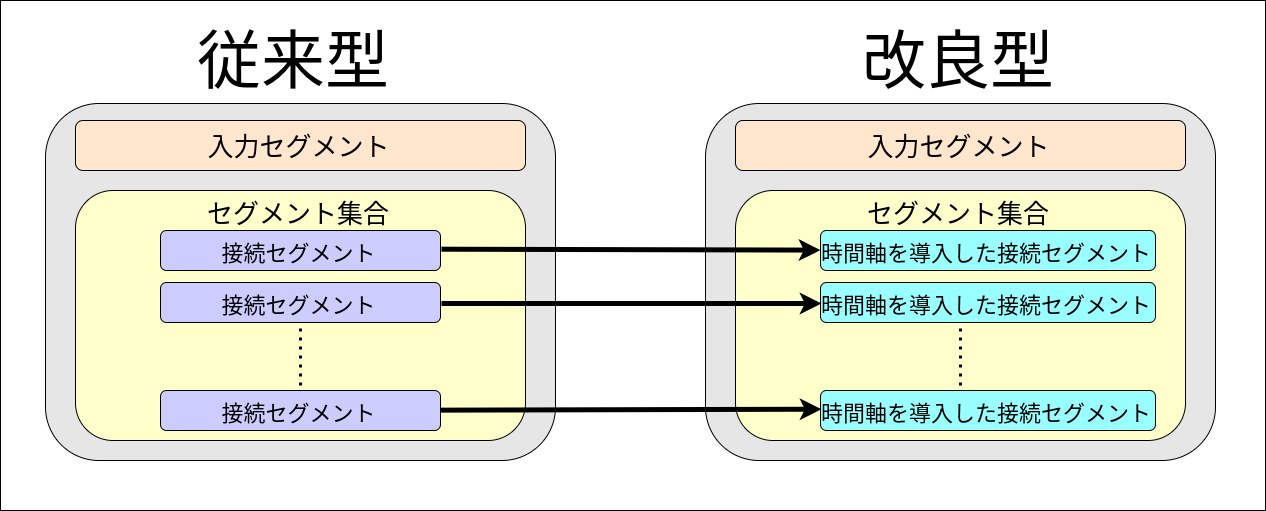
\includegraphics[width=14cm]{./fig/drawing_9}
    \caption{提案モデルにおけるセル内の構造}
    \label{fig:HTM_improved}
  \end{center}
\end{figure}

提案モデルのセル内の構造は以上のようになっている。
入力セグメントは従来型のHTMと同様になっているが、セグメント集合の構造は異なっている。
セグメント集合内の接続セグメントに関して時間軸を導入した。
これによって接続セグメントはHTM中のすべてのセルとの接続値と時間軸の3次元テンソル値となる。そのためセグメント集合は4次元のテンソル値となる。

\section{提案モデルの学習アルゴリズム}
提案モデルは従来のHTMを拡張しているため学習アルゴリズムにおいても拡張した部分がある。
時間軸を導入したことによって予測状態のセル計算とセグメント集合を用いた接続値の更新において変更点がある。

\subsubsection{従来型と同じ部分}

活性化状態のセルの計算に関しては従来のHTMと同様である。

\subsection{予測状態のセルの計算}
時間軸セグメントの長さを$\tau_c$とし、セグメント集合における接続値を${\bf D}^d_{ij}(\tau)$とする。
また接続値がしきい値を超えた値のみを取り出した接続の可否のみを表す2進行列を${\bf \tilde{D}}^d_{ij}(\tau)$とする。

\begin{equation}
  \pi^t_{ij} =
  \left\{
  \begin{alignedat}{2}
    1 \qquad &if \; \exists_\tau \exists_d\|{\bf \tilde{D}}^d_{ij}(\tau) \circ {\bf A^t}\|_1 > \theta \quad (t-\tau_c < \tau < t-1)\\
    0 \qquad &otherwise
  \end{alignedat}
  \right.
\end{equation}

\subsection{セグメント集合を用いた接続値の更新}
セグメントを更新する場合分けは従来型と同様となっている。
またセグメントの更新式も従来型と同様となっており式2.6と式2.7となっているが、セグメントの更新を複数の時間($t-\tau_c < t-1$)にわたって適用するように変更している。

\subsection{セグメント集合の大きさ}
改良型のHTMは従来型に比べてセグメント集合の次元が時間軸によって1次元拡張されているが、
セグメント集合を表すテンソルの大きさは一致するように調整している。
HTMにおけるセグメント集合の次元は従来型で3次元、改良型で4次元となっており、これが各セルごとに存在しているが、実装ではすべてのセルのセグメント集合をまとめて定義している。
これによってHTM全体でのセグメント集合は従来型で5次元、改良型で6次元となっている。
